\newpage
\section{SAR processing}

This section describes how to use the applications related to SAR processing.

\subsection{Calibration}

The application SarRadiometricCalibration can deal with the calibration of data from four radar sensors:
RadarSat2, Sentinel1, COSMO-SkyMed and TerraSAR-X.

Examples :

If SARimg.tif is a TerraSAR-X or a COSMO-SkyMed image :

\begin{verbatim} 
otbcli_SarRadiometricCalibration -in SARimg.tif -out
  SARimg-calibrated.tif 
\end{verbatim}
									  
If SARimg.tif is a RadarSat2 or a Sentinel1 image, it 's possible to specify the look-up table 
(automatically found in the metadata provided with such image) :

\begin{verbatim} 
otbcli_SarRadiometricCalibration -in SARimg.tif -lut gamma
									  -out
SARimg-calibrated.tif 
\end{verbatim}

For TerraSAR-X (and soon for RadarSat2 and Sentinel1), it is also possible
to use a noise LUT to derive calibrated noise profiles :

\begin{verbatim} 
otbcli_SarRadiometricCalibration -in SARimg.tif -lut gamma -noise 1
									  -out
SARimg-calibrated.tif 
\end{verbatim}

\subsection{Despeckle}
SAR images are generally corrupted by speckle noise. To suppress 
speckle and improve the radar image interpretability lots of filtering 
techniques have been proposed.  The module implements to well-known 
despeckle methods: Frost, Lee, Gamma-MAP and kuan.

The two figures below (\ref{fig:S1VVextractint} and \ref{fig:S1VVdespeckledextract}) show an extract of a SLC Sentinel1 image, band VV, taken over Cabo Verde.
The following commands were used to produce the despeckled extract :

First, the original image is converted into an intensity one (real part corresponds to band 1, and imaginary part to band 2):

\begin{verbatim} 
otbcli_BandMath -il S1-VV-extract.tif -exp im1b1^2+im1b2^2 -out
S1-VV-extract-int.tif 
\end{verbatim}

Then the intensity image is despeckled with the Gamma-MAP filter :

\begin{verbatim} 
otbcli_Despeckle -in S1-VV-extract-int.tif -filter.gammamap.rad 5
									   -filter.gammamap.nblooks
1 -out S1-VV-despeckled-extract.tif 
\end{verbatim}

The produced images were then rescaled to intensities ranging from 0 to 255 in order to be displayed.

\begin{center}
  \begin{figure}[h!]
    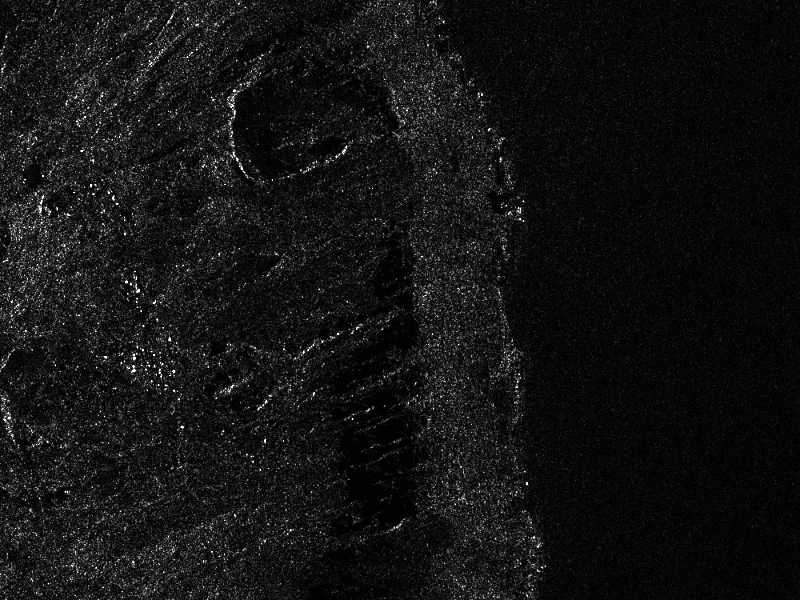
\includegraphics[width=\textwidth]{../Art/S1-VV-extract-int.png}
    \itkcaption[SAR despeckling]{Intensity image from a SLC-VV Sentinel1 image.}
    \label{fig:S1VVextractint}
   \end{figure}
   
   \begin{figure}[h!]
    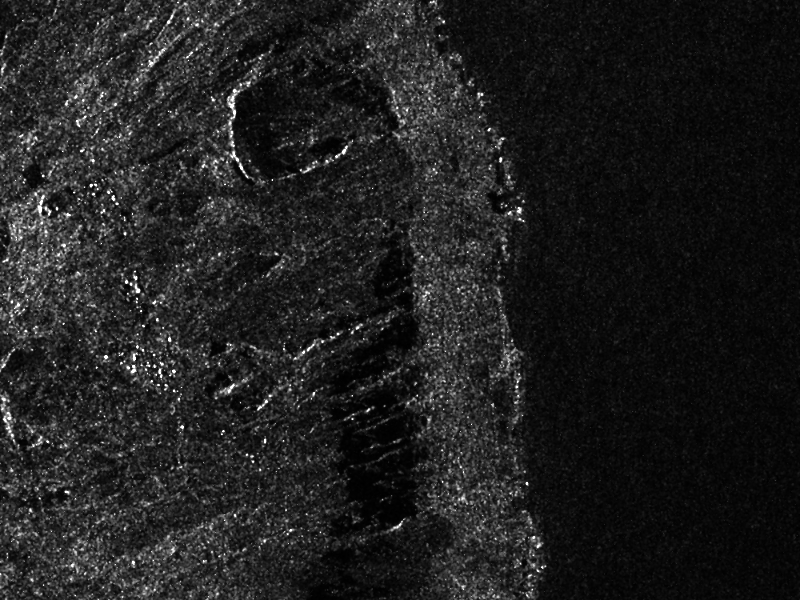
\includegraphics[width=\textwidth]{../Art/S1-VV-despeckled-extract.png}
    \itkcaption[SAR despeckling]{After despeckling with Gamma-Map filter.}
    \label{fig:S1VVdespeckledextract}
   \end{figure}
\end{center}


\subsection{Polarimetry}

In conventional imaging radar the measurement is a scalar which is 
proportional to the received backscattered power at a particular combination 
of linear polarization (HH, HV, VH or VV). 
Polarimetry is the measurement and interpretation of the polarization of this measurement which
allows to measure various optical properties of a material.
In polarimetry the basic measurement is a $2x2$ complex scattering
matrix yielding an eight dimensional measurement space (Sinclair
matrix). For reciprocal targets where $HV=VH$, this space is
compressed to five dimensions: three amplitudes ($|HH|$, $|HV|$, and
$|VV|$); and two phase measurements, (co-pol: HH-VV, and cross-pol:
HH-HV). (see \href{http://www.grss-ieee.org/technical-briefs/imaging-radar-polarimetry}{grss-ieee}).

\subsubsection{Matrix conversions}

This applications allows converting classical polarimetric matrices to each other.
For instance, it is possible to get the coherency matrix from the Sinclar one, or the Mueller matrix from the coherency one.
The figure below (\ref{fig:polconv}) shows the workflow used in this application.

\begin{figure}[h!]
  \centering
   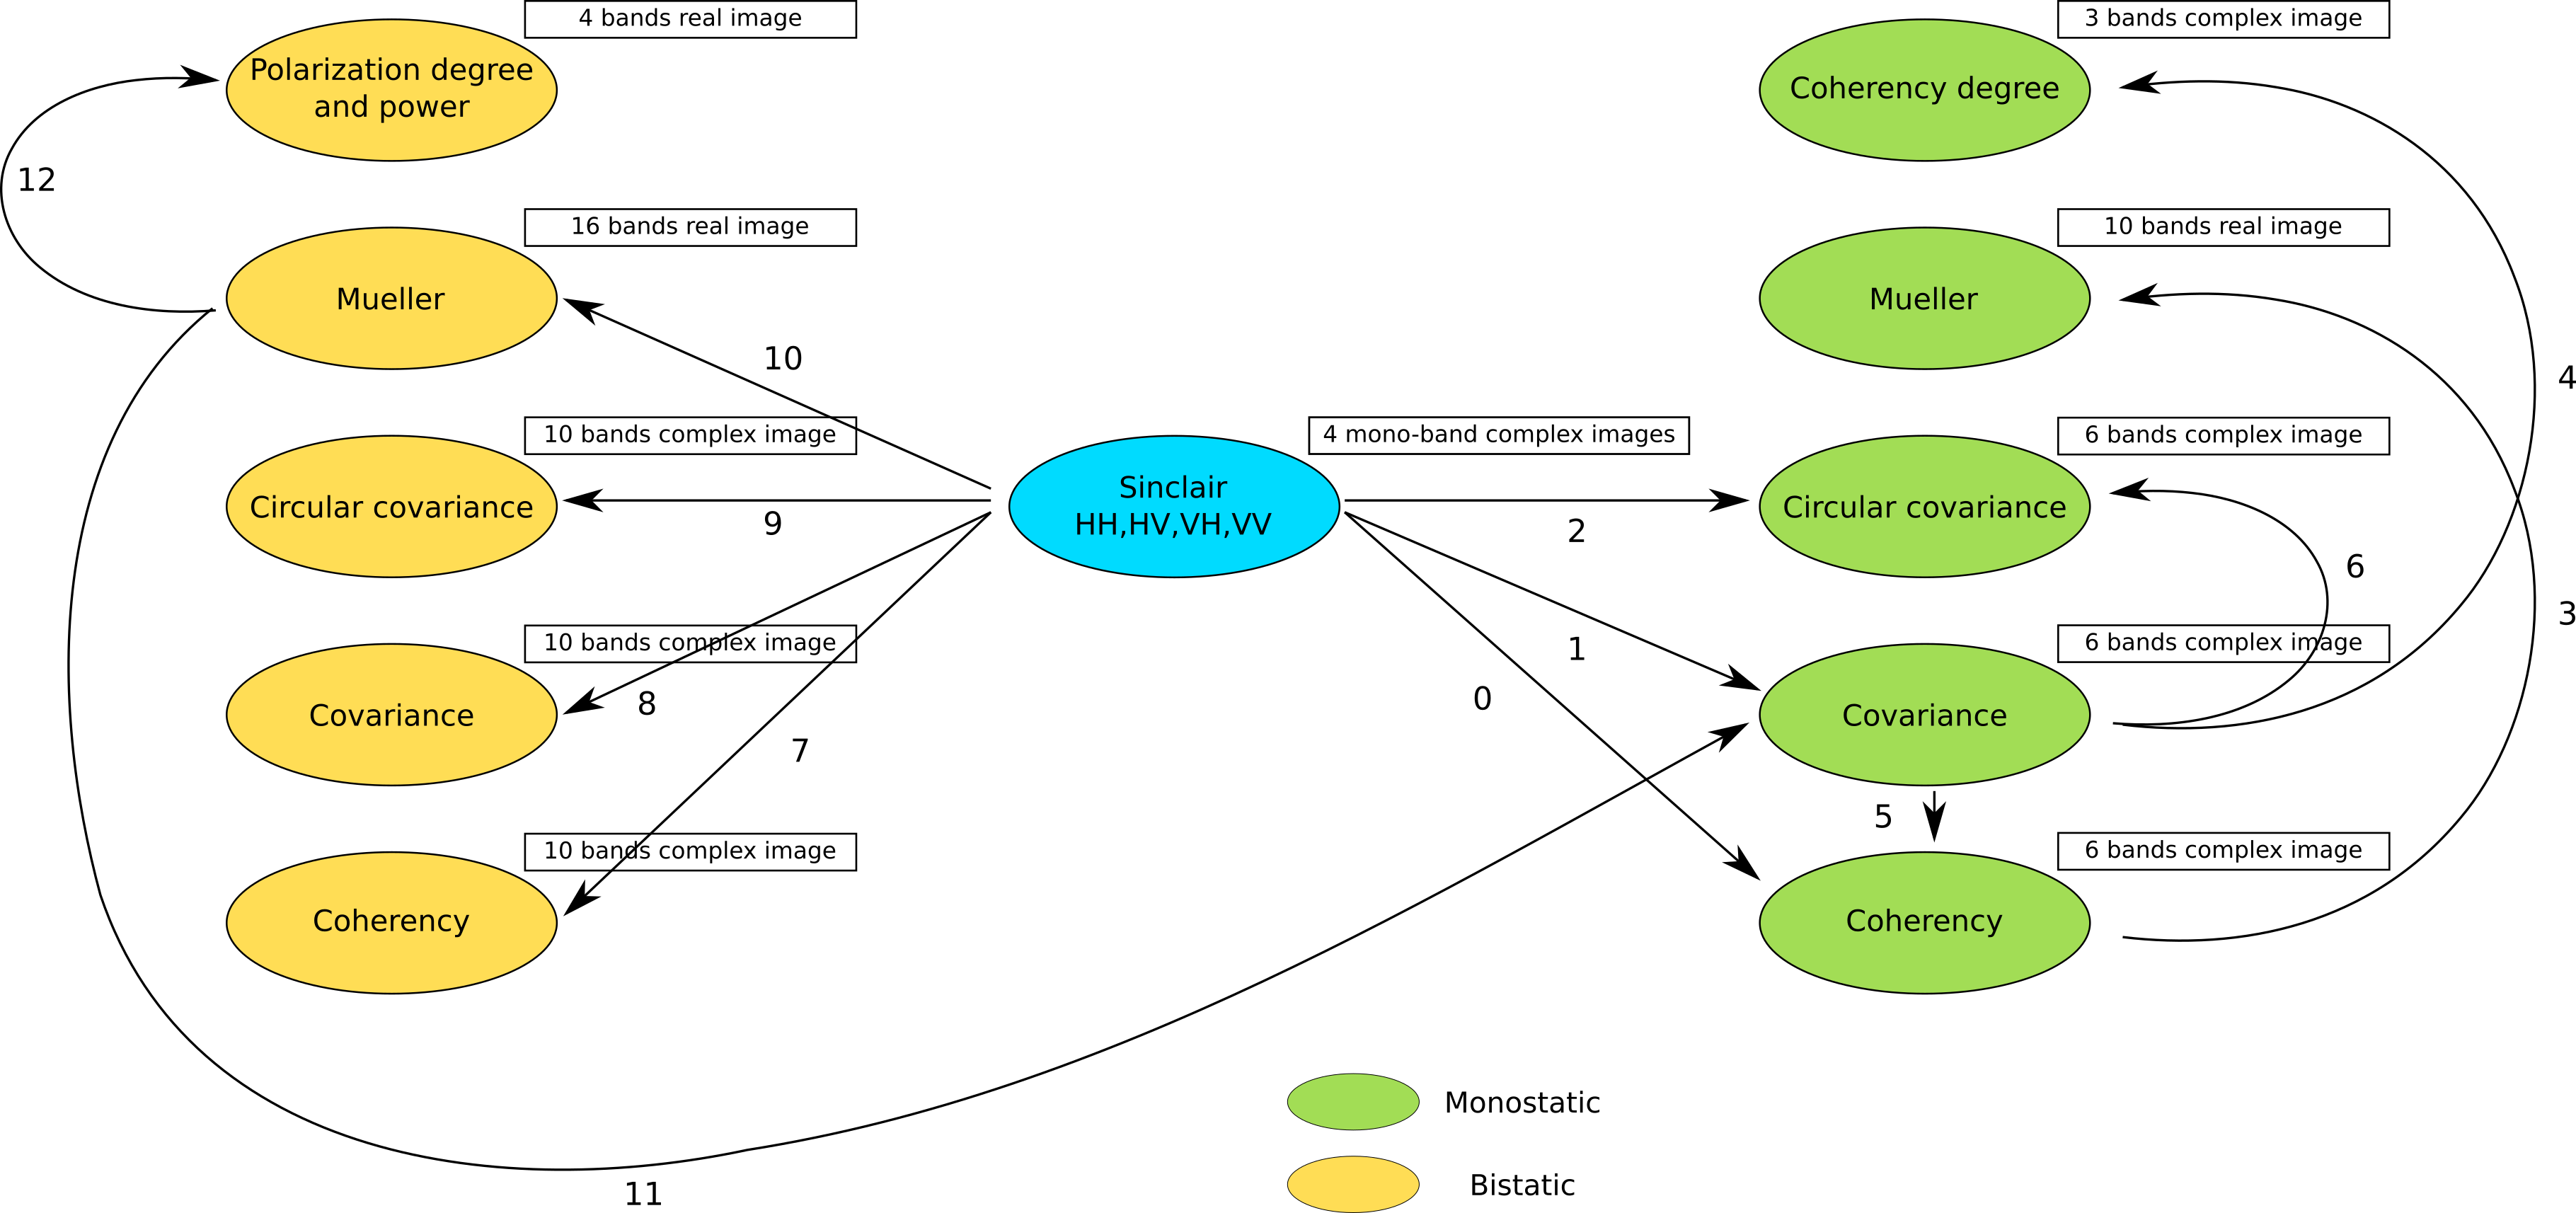
\includegraphics[width=\textwidth]{../Art/sarpol_conversion_schema.png}
  \itkcaption[SAR polarimetry conversion]{SAR polarimetry conversion application.}
  \label{fig:polconv}
\end{figure}

The filters used in this application never handle matrices, but images where each band is related to their elements.
As most of the time SAR polarimetry handles symetric matrices, only the relevant elements are stored, so that the images representing them have a minimal number of bands.
For instance, the coherency matrix size is 3x3 in the monostatic case, and 4x4 in the bistatic case : it will thus be stored in a 6-band or a 10-band complex image (the diagonal and the upper elements of the matrix).

The Sinclair matrix is a special case : it is always represented as 3 or 4 one-band complex images (for mono- or bistatic case).

There are 13 available conversions, each one being related to the following  parameters:
\begin{enumerate}
\item msinclairtocoherency
\item msinclairtocovariance
\item msinclairtocircovariance
\item mcoherencytomueller
\item mcovariancetocoherencydegree
\item mcovariancetocoherency
\item mlinearcovariancetocircularcovariance
\item muellertomcovariance
\item bsinclairtocoherency
\item bsinclairtocovariance
\item bsinclairtocircovariance
\item sinclairtomueller
\item muellertopoldegandpower
\end{enumerate}

For each option parameter, the list below gives the formula used.

--- Monostatic case ---

\begin{enumerate}
\renewcommand{\labelenumii}{Channel \arabic{enumii} : }
\item msinclairtocoherency (SinclairToReciprocalCoherencyMatrixFunctor)
\begin{enumerate}
\item $ 0.5 . (S_{hh}+S_{vv}).(S_{hh}+S_{vv})^{*} $
\item $ 0.5 . (S_{hh}+S_{vv}).(S_{hh}-S_{vv})^{*} $
\item $ 0.5 . (S_{hh}+S_{vv}).(2 S_{hv})^{*} $
\item $ 0.5 . (S_{hh}-S_{vv}).(S_{hh}-S_{vv})^{*} $
\item $ 0.5 . (S_{hh}-S_{vv}).(2 S_{hv})^{*} $
\item $ 0.5 . (2 S_{hv}).(2 S_{hv})^{*} $
\end{enumerate}
 
\item msinclairtocovariance (SinclairToReciprocalCovarianceMatrixFunctor)
\begin{enumerate}
\item $ S_{hh}.S_{hh}^{*} $ 
\item $ \sqrt{2}.S_{hh}.S_{hv}^{*} $ 
\item $ S_{hh}.S_{vv}^{*} $ 
\item $ 2.S_{hv}.S_{hv}^{*} $ 
\item $ \sqrt{2}.S_{hv}.S_{vv}^{*} $ 
\item $ S_{vv}.S_{vv}^{*} $
\end{enumerate}
 
\item msinclairtocircovariance (SinclairToReciprocalCircularCovarianceMatrixFunctor)
\begin{enumerate}
\item $ S_{ll}.S_{ll}^{*} $ 
\item $ S_{ll}.S_{lr}^{*} $ 
\item $ S_{ll}.S_{rr}^{*} $ 
\item $ S_{lr}.S_{lr}^{*} $ 
\item $ S_{lr}.S_{rr}^{*} $ 
\item $ S_{rr}.S_{rr}^{*} $
\end{enumerate}

With:
\begin{itemize} 
\item $ S_{ll} = 0.5(S_{hh}+2j S_{hv}-S_{vv}) $ 
\item $ S_{lr} = 0.5(j S_{hh}+j S_{vv}) $  
\item $ S_{rr} = 0.5(-S_{hh}+2j S_{hv}+S_{vv}) $ 
\end{itemize}
 
\item mcoherencytomueller (ReciprocalCoherencyToReciprocalMuellerFunctor)
\begin{enumerate}
\item $ 0.5*( C_{11}+C_{22}+C_{33} ) $ 
\item $ Re(C_{12}) + Im(C_{22}) $ 
\item $ Re(C_{13}) $ 
\item $ Im(C_{23}) $ 
\item $ Re(C_{12}) $ 
\item $ 0.5*( C_{11}+C_{22}-C_{33} ) $ 
\item $ Re(C_{23}) $ 
\item $ Im(C_{13}) $ 
\item $ -Re(C_{13}) $ 
\item $ -Re(C_{23}) $
\item $ 0.5.Re(VAL1) $
\item $ 0.5.Im(VAL0) $
\item $ Im(C_{23}) $
\item $ Im(C_{13}) $
\item $ 0.5.Im(VAL1^{*}) $
\item $ 0.5.Re(VAL0) $
\end{enumerate}

With:
\begin{itemize} 
\item $ VAL0 = C_{33}+C_{12}-C_{11}-(C_{12}-C_{22})^{*}  $ 
\item $ VAL1 = -C_{33}+C_{12}-C_{11}-(C_{12}-C_{22})^{*} $ 
\end{itemize}

Where Cij are related to the elements of the reciprocal coherence matrix.
 
 
\item mcovariancetocoherencydegree (ReciprocalCovarianceToCoherencyDegreeFunctor)
\begin{enumerate}
\item $ abs(S_{hh}.S_{vv}^{*}) / sqrt(S_{hh}.S_{hh}^{*}) / sqrt(S_{vv}.S_{vv}^{*}) $ 
\item $ abs(S_{hv}.S_{vv}^{*}) / sqrt(S_{hv}.S_{hv}^{*}) / sqrt(S_{vv}.S_{vv}^{*}) $ 
\item $ abs(S_{hh}.S_{hv}^{*}) / sqrt(S_{hh}.S_{hh}^{*}) / sqrt(S_{hv}.S_{hv}^{*}) $
\end{enumerate}
 
\item mcovariancetocoherency (ReciprocalCovarianceToReciprocalCoherencyFunctor)
\begin{enumerate}
\item $ 0.5 . ( C_{33} + C_{13} + C_{13}^{*} + C_{11} ) $ 
\item $ 0.5 . ( -C_{33} - C_{13} + C_{13}^{*} + C_{11} ) $ 
\item $ 0.5 . ( \sqrt{2}.C_{12} + \sqrt{2}.C_{23}^{*} ) $ 
\item $ 0.5 . ( C_{33} - C_{13} - C_{13}^{*} + C_{11} ) $ 
\item $ 0.5 . ( \sqrt{2}.C_{12} - \sqrt{2}.C_{23}^{*} ) $ 
\item $ 0.5 . ( 2 . C_{22} ) $
\end{enumerate}

Where Cij are related to the elements of the reciprocal linear covariance matrix.
 
\item mlinearcovariancetocircularcovariance (ReciprocalLinearCovarianceToReciprocalCircularCovarianceFunctor)
\begin{enumerate}
\item $ 0.25 . ( C_{33}-i.\sqrt{2}.C_{23}-C_{13}+i.\sqrt{2}.C_{23}^{*}-C_{13}^{*}+2.C_{22}-i.\sqrt{2}.C_{12}+i.\sqrt{2}.C_{12}^{*}+C_{11} ) $ 
\item $ 0.25 . ( i.\sqrt{2}.C_{33}+2.C_{23}-i.\sqrt{2}.C_{13}+i.\sqrt{2}.C_{13}^{*}+2.C_{12}^{*}-i.\sqrt{2}.C_{11} ) $ 
\item $ 0.25 . ( -C_{33}+i.\sqrt{2}.C_{23}+C_{13}+i.\sqrt{2}.C_{23}^{*}+C_{13}^{*}+2.C_{22}-i.\sqrt{2}.C_{12}-i.\sqrt{2}.C_{12}^{*}-C_{11} ) $ 
\item $ 0.25 . ( 2.C_{33}+2.C_{13}+2.C_{13}^{*}+2.C_{11} ) $ 
\item $ 0.25 . ( i.\sqrt{2}.C_{33}+i.\sqrt{2}.C_{13}+2.C_{23}^{*}-i.\sqrt{2}.C_{13}^{*}+2.C_{12}-i.\sqrt{2}.C_{11} ) $ 
\item $ 0.25 . ( C_{33}+i.\sqrt{2}.C_{23}-C_{13}-i.\sqrt{2}.C_{23}^{*}-C_{13}^{*}+2.C_{22}+i.\sqrt{2}.C_{12}-i.\sqrt{2}.C_{12}^{*}+C_{11} ) $
\end{enumerate}

Where Cij are related to the elements of the reciprocal linear covariance matrix.

\item muellertomcovariance (MuellerToReciprocalCovarianceFunctor)
\begin{enumerate}
\item $ 0.5.(M_{11}+M_{22}+2.M_{12}) $ 
\item $ 0.5.\sqrt{2}.[(M_{13}+M_{23}) + j.(M_{14}+M_{24})] $ 
\item $ -0.5.(M_{33}+M_{44}) - j.M_{34} $ 
\item $ M_{11}-M_{22} $ 
\item $ 0.5.\sqrt{2}.[(M_{13}-M_{23}) + j.(M_{14}-M_{24})] $ 
\item $ 0.5.(M_{11}+M_{22}-2.M_{12}) $
\end{enumerate}

\end{enumerate}

--- Bistatic case ---

\begin{enumerate}
\renewcommand{\labelenumii}{Channel \arabic{enumii} : }
\setcounter{enumi}{8}

\item bsinclairtocoherency (SinclairToCoherencyMatrixFunctor)
\begin{enumerate}
\item $ (S_{hh}+S_{vv}).(S_{hh}+S_{vv})^{*} $ 
\item $ (S_{hh}+S_{vv}).(S_{hh}-S_{vv})^{*} $ 
\item $ (S_{hh}+S_{vv}).(S_{hv}+S_{vh})^{*} $ 
\item $ (S_{hh}+S_{vv}).( j (S_{hv}-S_{vh}))^{*} $ 
\item $ (S_{hh}-S_{vv}).(S_{hh}-S_{vv})^{*} $ 
\item $ (S_{hh}-S_{vv}).(S_{hv}+S_{vh})^{*} $ 
\item $ (S_{hh}-S_{vv}).( j (S_{hv}-S_{vh}))^{*} $ 
\item $ (S_{hv}+S_{vh}).(S_{hv}+S_{vh})^{*} $ 
\item $ (S_{hv}+S_{vh}).( j (S_{hv}-S_{vh}))^{*} $ 
\item $ j (S_{hv}-S_{vh}).( j (S_{hv}-S_{vh}))^{*} $
\end{enumerate}
 
\item bsinclairtocovariance (SinclairToCovarianceMatrixFunctor)
\begin{enumerate}
\item $ S_{hh}.S_{hh}^{*} $ 
\item $ S_{hh}.S_{hv}^{*} $ 
\item $ S_{hh}.S_{vh}^{*} $ 
\item $ S_{hh}.S_{vv}^{*} $ 
\item $ S_{hv}.S_{hv}^{*} $ 
\item $ S_{hv}.S_{vh}^{*} $ 
\item $ S_{hv}.S_{vv}^{*} $ 
\item $ S_{vh}.S_{vh}^{*} $ 
\item $ S_{vh}.S_{vv}^{*} $ 
\item $ S_{vv}.S_{vv}^{*} $
\end{enumerate}
 
\item bsinclairtocircovariance (SinclairToCircularCovarianceMatrixFunctor)
\begin{enumerate}
\item $ S_{ll}.S_{ll}^{*} $ 
\item $ S_{ll}.S_{lr}^{*} $ 
\item $ S_{ll}.S_{rl}^{*} $ 
\item $ S_{ll}.S_{rr}^{*} $ 
\item $ S_{lr}.S_{lr}^{*} $ 
\item $ S_{lr}.S_{rl}^{*} $ 
\item $ S_{lr}.S_{rr}^{*} $ 
\item $ S_{rl}.S_{rl}^{*} $ 
\item $ S_{rl}.S_{rr}^{*} $ 
\item $ S_{rr}.S_{rr}^{*} $ 
\end{enumerate}

With:
\begin{itemize} 
\item $ S_{ll} = 0.5(S_{hh}+j S_{hv}+j S_{vh}-S_{vv}) $ 
\item $ S_{lr} = 0.5(j S_{hh}+S_{hv}-S_{vh}+j S_{vv}) $ 
\item $ S_{rl} = 0.5(j S_{hh}-S_{hv}+ S_{vh}+j S_{vv}) $ 
\item $ S_{rr} = 0.5(-S_{hh}+j S_{hv}+j S_{vh}+S_{vv}) $ 
\end{itemize}
 


--- Both cases ---

\item sinclairtomueller (SinclairToMueller)
\begin{enumerate} 
\item $ 0.5 Re( T_{xx}.T_{xx}^{*} + T_{xy}.T_{xy}^{*} + T_{yx}.T_{yx}^{*} + T_{yy}.T_{yy}^{*} ) $ 
\item $ 0.5 Re( T_{xx}.T_{xx}^{*} - T_{xy}.T_{xy}^{*} + T_{yx}.T_{yx}^{*} - T_{yy}.T_{yy}^{*} ) $ 
\item $ Re( T_{xx}.T_{xy}^{*} + T_{yx}.T_{yy}^{*} ) $ 
\item $ Im( T_{xx}.T_{xy}^{*} + T_{yx}.T_{yy}^{*} ) $ 
\item $ 0.5 Re( T_{xx}.T_{xx}^{*} + T_{xy}.T_{xy}^{*} - T_{yx}.T_{yx}^{*} - T_{yy}.T_{yy}^{*} ) $ 
\item $ 0.5 Re( T_{xx}.T_{xx}^{*} - T_{xy}.T_{xy}^{*} - T_{yx}.T_{yx}^{*} + T_{yy}.T_{yy}^{*} ) $ 
\item $ Re( T_{xx}.T_{xy}^{*} - T_{yx}.T_{yy}^{*} ) $ 
\item $ Im( T_{xx}.T_{xy}^{*} - T_{yx}.T_{yy}^{*} ) $ 
\item $ Re( T_{xx}.T_{yx}^{*} + T_{xy}.T_{yy}^{*} ) $ 
\item $ Im( T_{xx}.T_{yx}^{*} - T_{xy}.T_{yy}^{*} ) $ 
\item $ Re( T_{xx}.T_{yy}^{*} + T_{xy}.T_{yx}^{*} ) $ 
\item $ Im( T_{xx}.T_{yy}^{*} - T_{xy}.T_{yx}^{*} ) $ 
\item $ Re( T_{xx}.T_{yx}^{*} + T_{xy}.T_{yy}^{*} ) $ 
\item $ Im( T_{xx}.T_{yx}^{*} - T_{xy}.T_{yy}^{*} ) $ 
\item $ Re( T_{xx}.T_{yy}^{*} + T_{xy}.T_{yx}^{*} ) $ 
\item $ Im( T_{xx}.T_{yy}^{*} - T_{xy}.T_{yx}^{*} ) $
\end{enumerate}

With :
\begin{itemize}
\item $ T_{xx} = -S_{hh} $ 
\item $ T_{xy} = -S_{hv} $ 
\item $ T_{yx} = S_{vh} $ 
\item $ T_{yy} = S_{vv} $ 
\end{itemize}

 
\item muellertopoldegandpower (MuellerToPolarisationDegreeAndPowerFunctor)
\begin{enumerate}
\item $ P_{min} $ 
\item $ P_{max} $ 
\item $ DegP_{min} $ 
\item $ DegP_{max} $
\end{enumerate}

\end{enumerate}

Examples :

\begin{enumerate}
\item 
\begin{verbatim} 
otbcli_SARPolarMatrixConvert -inhh imageryC_HH.tif -inhv imageryC_HV.tif -invv imageryC_VV.tif
									  -conv
                                                                          msinclairtocoherency
                                                                          -outc
                                                                          coherency.tif 
\end{verbatim}
									  
\item 
\begin{verbatim} 
otbcli_SARPolarMatrixConvert -inhh imageryC_HH.tif -inhv imageryC_HV.tif -invv imageryC_VV.tif
									  -conv
                                                                          msinclairtocovariance
                                                                          -outc
                                                                          covariance.tif 
\end{verbatim}
									  
\item 
\begin{verbatim} 
otbcli_SARPolarMatrixConvert -inhh imageryC_HH.tif -inhv imageryC_HV.tif -invv imageryC_VV.tif
									  -conv
                                                                          msinclairtocircovariance
                                                                          -outc
                                                                          circ_covariance.tif 
\end{verbatim}
									  
\item 
\begin{verbatim} 
otbcli_SARPolarMatrixConvert -inc coherency.tif 
									  -conv
                                                                          mcoherencytomueller
                                                                          -outf
                                                                          mueller.tif 
\end{verbatim}
									  
\item 
\begin{verbatim} 
otbcli_SARPolarMatrixConvert -inc covariance.tif 
									  -conv
                                                                          mcovariancetocoherencydegree
                                                                          -outc
                                                                          coherency_degree.tif 
\end{verbatim}
									  
\item 
\begin{verbatim} 
otbcli_SARPolarMatrixConvert -inc covariance.tif 
									  -conv
                                                                          mcovariancetocoherency
                                                                          -outc
                                                                          coherency.tif 
\end{verbatim}
									  
\item 
\begin{verbatim} 
otbcli_SARPolarMatrixConvert -inc covariance.tif 
									  -conv
                                                                          mlinearcovariancetocircularcovariance
                                                                          -outc
                                                                          circ_covariance.tif 
\end{verbatim}	
									  			
\item 
\begin{verbatim} 
otbcli_SARPolarMatrixConvert -inf mueller.tif 
									  -conv
                                                                          muellertomcovariance
                                                                          -outc
                                                                          covariance.tif 
\end{verbatim}	
									  								  
\item 
\begin{verbatim} 
otbcli_SARPolarMatrixConvert -inhh imageryC_HH.tif -inhv imageryC_HV.tif -invh imageryC_VH.tif -invv imageryC_VV.tif
									  -conv
                                                                          bsinclairtocoherency
                                                                          -outc
                                                                          bcoherency.tif 
\end{verbatim}
									  
\item 
\begin{verbatim} 
otbcli_SARPolarMatrixConvert -inhh imageryC_HH.tif -inhv imageryC_HV.tif -invh imageryC_VH.tif -invv imageryC_VV.tif 
									  -conv
                                                                          bsinclairtocovariance
                                                                          -outc
                                                                          bcovariance.tif 
\end{verbatim}
									  
\item 
\begin{verbatim} 
otbcli_SARPolarMatrixConvert -inhh imageryC_HH.tif -inhv imageryC_HV.tif -invh imageryC_VH.tif -invv imageryC_VV.tif
									  -conv
                                                                          bsinclairtocircovariance
                                                                          -outc
                                                                          circ_bcovariance.tif 
\end{verbatim}
									  
									  
\item 
\begin{verbatim} 
otbcli_SARPolarMatrixConvert -inhh imageryC_HH.tif -inhv imageryC_HV.tif -invh imageryC_VH.tif -invv imageryC_VV.tif 
									  -conv
                                                                          sinclairtomueller
                                                                          -outf
                                                                          mueller.tif 
\end{verbatim}
									  
\item 
\begin{verbatim} 
otbcli_SARPolarMatrixConvert -inf mueller.tif 
									  -conv
                                                                          muellertopoldegandpower
                                                                          -outf
                                                                          degreepower.tif 
\end{verbatim}
									  
\end{enumerate}

\subsubsection{Polarimetric decompositions}

From one-band complex images (HH, HV, VH, VV), returns the selected decomposition.
The H-alpha-A decomposition is currently the only one available; it is implemented for the monostatic case (transmitter and receiver are co-located).
User must provide three one-band complex images HH, HV or VH, and VV (HV = VH in monostatic case).
The H-alpha-A decomposition consists in averaging 3x3 complex coherency matrices (incoherent analysis) : 
The user must provide the size of the averaging window, thanks to the parameter inco.kernelsize.
The applications returns a float vector image, made of three channels : H (entropy), Alpha, A (Anisotropy).

Here are the formula used (refer to the previous section about how the coherence matrix is obtained from the sinclair one):
\begin{enumerate}
\renewcommand{\labelenumii}{Channel \arabic{enumii} : }
\item $ entropy = -\sum_{i=0}^{2} \frac{p[i].\log{p[i]}}{\log{3}} $
\item $ \alpha = \sum_{i=0}^{2} p[i].\alpha_{i} $
\item $ anisotropy = \frac {SortedEigenValues[1] - SortedEigenValues[2]}{SortedEigenValues[1] + SortedEigenValues[2]} $
\end{enumerate}

Where:
\begin{itemize}
\item $ p[i] = max(SortedEigenValues[i], 0) / \sum_{i=0}^{2, SortedEigenValues[i]>0} SortedEigenValues[i] $
\item $ \alpha_{i} = \left| SortedEigenVector[i] \right|* \frac{180}{\pi}$
\end{itemize}


Example :

We first extract a ROI from the original image (not required). 
Here imagery\_HH.tif represents the element HH of the Sinclair matrix (and so forth).

\begin{itemize}
\item 
\begin{verbatim} 
otbcli_ExtractROI -in imagery_HH.tif -out imagery_HH_extract.tif  
									  -startx
0 -starty 0 -sizex 1000 -sizey 1000 
\end{verbatim}
									  
\item 
\begin{verbatim} 
otbcli_ExtractROI -in imagery_HV.tif -out imagery_HV_extract.tif  
									  -startx
                                                                          0
                                                                          -starty
                                                                          0
                                                                          -sizex
                                                                          1000
                                                                          -sizey
                                                                          1000 
\end{verbatim}
									  
\item 
\begin{verbatim} 
otbcli_ExtractROI -in imagery_VV.tif -out imagery_VV_extract.tif  
									  -startx
                                                                          0
                                                                          -starty
                                                                          0
                                                                          -sizex
                                                                          1000
                                                                          -sizey
                                                                          1000 
\end{verbatim}
\end{itemize}

Next we apply the H-alpha-A decomposition :

\begin{verbatim} 
otbcli_SARDecompositions -inhh imagery_HH_extract.tif -inhv imagery_HV_extract.tif -invv imagery_VV_extract.tif 
					-decomp haa -inco.kernelsize 5 -out
haa_extract.tif 
\end{verbatim}

The result is made uo of 3 bands : entropy (0..1) - alpha (0..90) - anisotropy (0..1). 
It is splitted into 3 mono-band images thanks to following command :

\begin{verbatim} 
otbcli_SplitImage -in haa_extract.tif -out
  haa_extract_splitted.tif 
\end{verbatim}

Each image is then colored thanks to a color look-up table 'hot'. 
Notice the way extremal values are provided for each polarimetric variable.

\begin{itemize}
\item 
\begin{verbatim} 
otbcli_ColorMapping -in haa_extract_splitted_0.tif -method continuous 
    -method.continuous.lut hot -method.continuous.min 0 -method.continuous.max 1
-out entropy_hot.tif uint8 
\end{verbatim}
									  
\item 
\begin{verbatim} 
otbcli_ColorMapping -in haa_extract_splitted_1.tif -method continuous 
    -method.continuous.lut hot -method.continuous.min 0 -method.continuous.max
    90 -out alpha_hot.tif uint8 
\end{verbatim}
									  
\item 
\begin{verbatim} 
otbcli_ColorMapping -in haa_extract_splitted_2.tif -method continuous 
    -method.continuous.lut hot -method.continuous.min 0 -method.continuous.max 1
    -out anisotropy_hot.tif uint8 
\end{verbatim}
\end{itemize}

The results are shown in the figures below (\ref{fig:entropyimage} , \ref{fig:alphaimage} and \ref{fig:anisotropyimage}).

\begin{center}
  \begin{figure}[h!]
    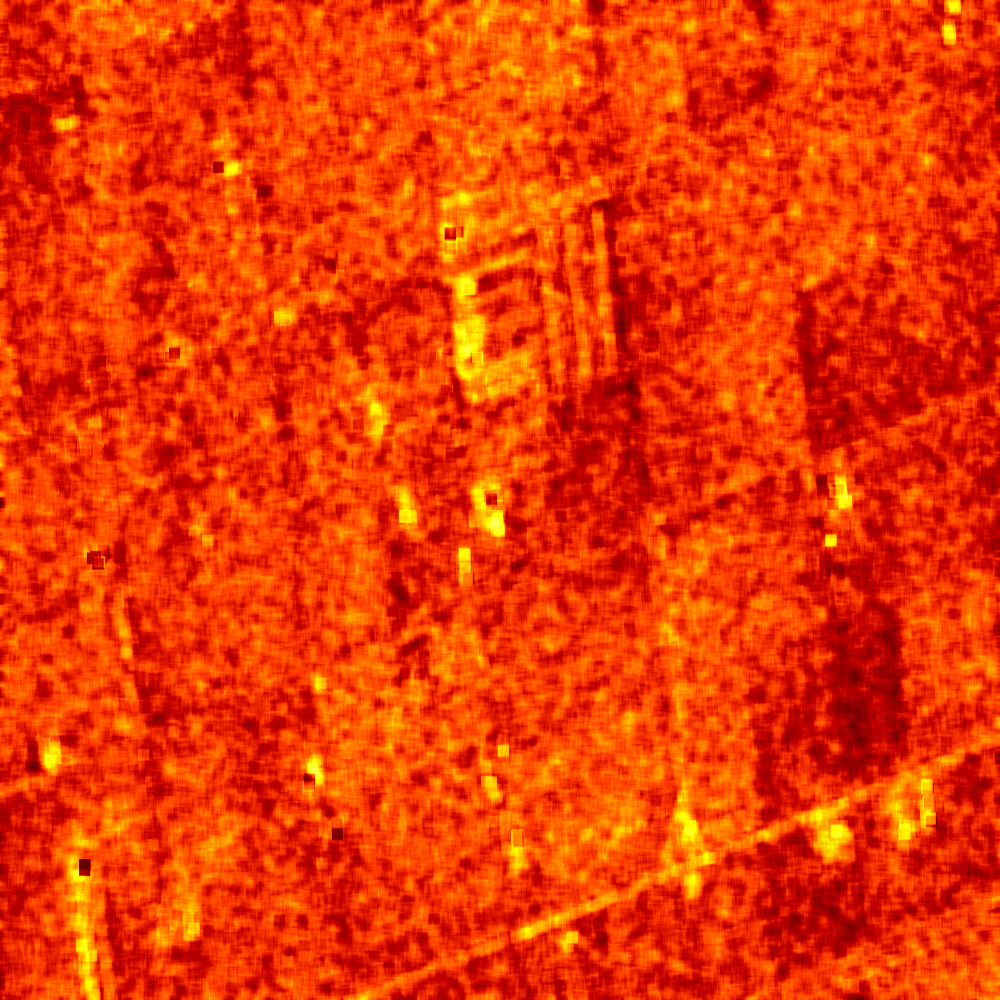
\includegraphics[width=\textwidth]{../Art/entropyhot.png}
    \itkcaption[SAR decomp]{Entropy image.}
    \label{fig:entropyimage}
   \end{figure}
   
   \begin{figure}[h!]
    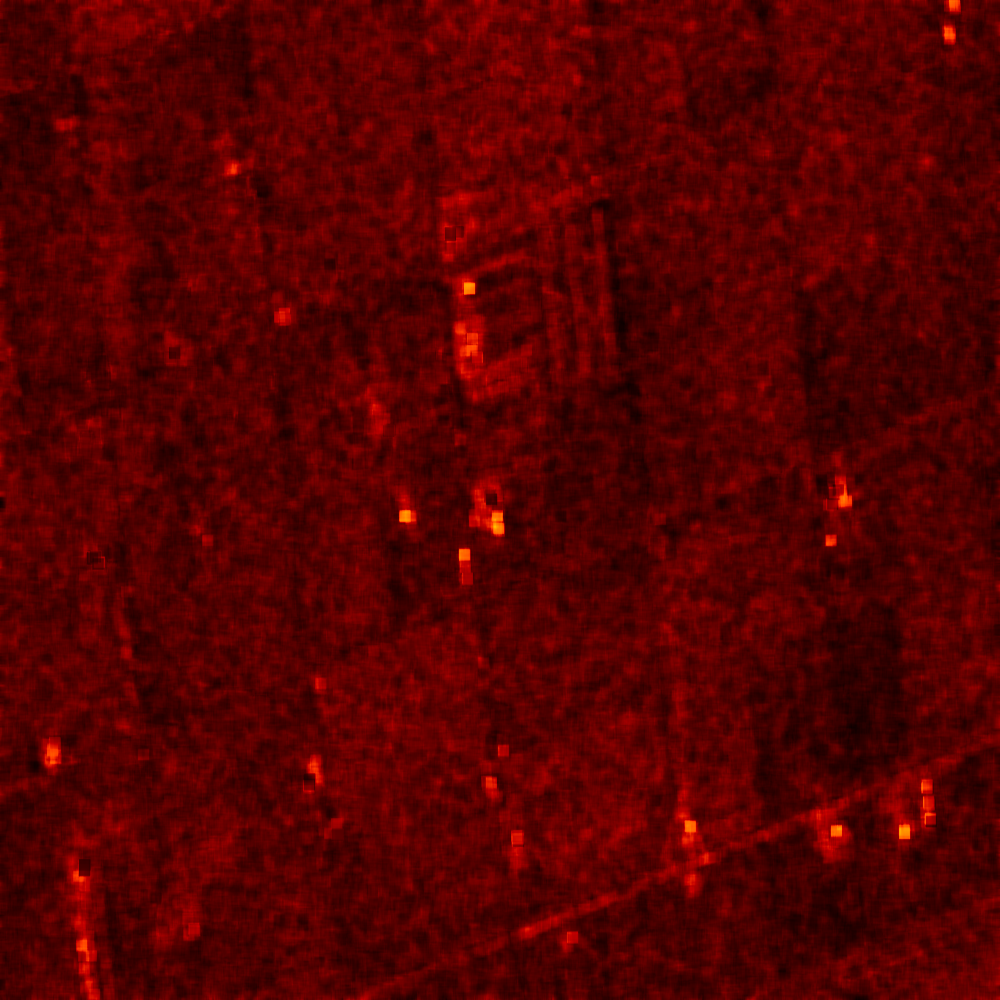
\includegraphics[width=\textwidth]{../Art/alphahot.png}
    \itkcaption[SAR decomp]{Alpha image.}
    \label{fig:alphaimage}
   \end{figure}
   
    \begin{figure}[h!]
    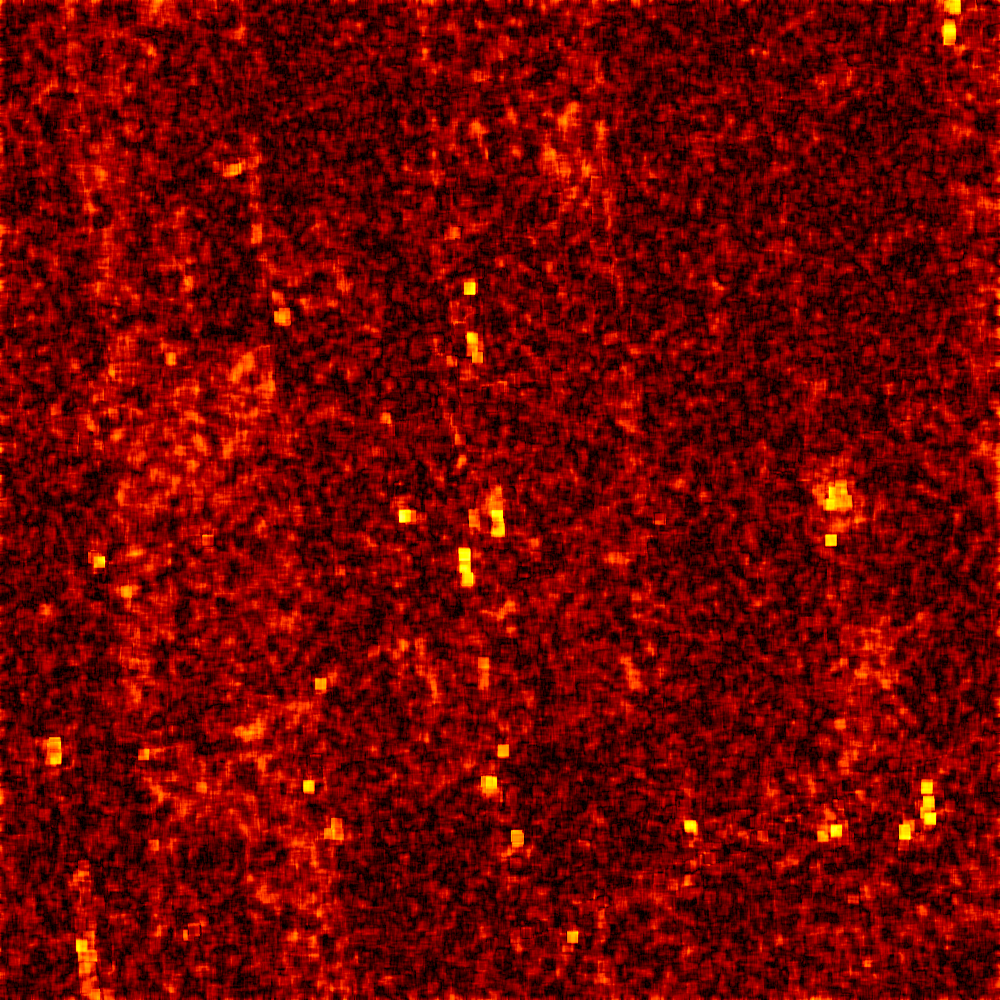
\includegraphics[width=\textwidth]{../Art/anisotropyhot.png}
    \itkcaption[SAR decomp]{Anisotropy image.}
    \label{fig:anisotropyimage}
   \end{figure}
   
\end{center}



\subsubsection{Polarimetric synthetis}

This application gives, for each pixel, the power that would have been received by a SAR system with a basis different from the classical (H,V) one (polarimetric synthetis). 
The new basis are indicated through two Jones vectors, defined by the user thanks to orientation (psi) and ellipticity (khi) parameters.
These parameters are namely psii, khii, psir and khir. The suffixes (i) and (r) refer to the transmiting antenna and the receiving antenna respectively.
Orientations and ellipticities are given in degrees, and are between -90/90 degrees and -45/45 degrees respectively. 

Four polarization architectures can be processed :
\begin{enumerate}
\item HH\_HV\_VH\_VV : full polarization, general bistatic case.
\item HH\_HV\_VV or HH\_VH\_VV : full polarization, monostatic case (transmitter and receiver are co-located).
\item HH\_HV : dual polarization.
\item VH\_VV : dual polarization.
\end{enumerate}
The application takes a complex vector image as input, where each band correspond to a particular emission/reception polarization scheme.
User must comply with the band order given above, since the bands are used to build the Sinclair matrix.

In order to determine the architecture, the application first relies on the number of bands of the input image.
\begin{enumerate}
\item Architecture HH\_HV\_VH\_VV is the only one with four bands, there is no possible confusion.
\item Concerning HH\_HV\_VV and HH\_VH\_VV architectures, both correspond to a three channels image. But they are processed in the same way, as the Sinclair matrix is symetric in the monostatic case.
\item Finally, the two last architectures (dual polarizations), can't be distinguished only by the number of bands of the input image. User must then use the parameters emissionh and emissionv to indicate the architecture of the system : emissionh=1 and emissionv=0 for HH\_HV,  emissionh=0 and emissionv=1 for VH\_VV.
\end{enumerate}
Note : if the architecture is HH\_HV, khii and psii are automatically set to 0/0 degrees; if the architecture is VH\_VV, khii and psii are automatically set to 0/90 degrees.

It is also possible to force the calculation to co-polar or cross-polar modes.
In the co-polar case, values for psir and khir will be ignored and forced to psii and khii; same as the cross-polar mode, where khir and psir will be forced to psii + 90 degrees and -khii.

Finally, the result of the polarimetric synthetis is expressed in the power domain, through a one-band scalar image. \newline


 
The final formula is thus : $P=\mid B^T.[S].A\mid^2$ , where A ans B are two Jones vectors and S is a Sinclair matrix.
 
The two figures below (\ref{fig:polsynthll} and \ref{fig:polsynthlr}) show the two images obtained with the basis LL and LR (L for left circular polarization and R for right polarization),
from a Radarsat 2 image taken over Vancouver. Once the four two-band images imagery\_HH imagery\_HV imagery\_VH imagery\_VV were merged 
into a single four complex band image imageryC\_HH\_HV\_VH\_VV.tif, the following commands were used to produce the LL and LR images :

\begin{verbatim} 
otbcli_SARPolarSynth -in imageryC_HH_HV_VH_VV.tif 
									  -psii
0 -khii 45 -mode co -out test-LL.tif 
\end{verbatim}
\begin{verbatim} 
otbcli_SARPolarSynth -in imageryC_HH_HV_VH_VV.tif 
									  -psii
0 -khii 45 -mode cross -out test-LR.tif 
\end{verbatim}

The produced images were then rescaled to intensities ranging from 0 to 255 in order to be displayed.


\begin{center}
  \begin{figure}[h!]
    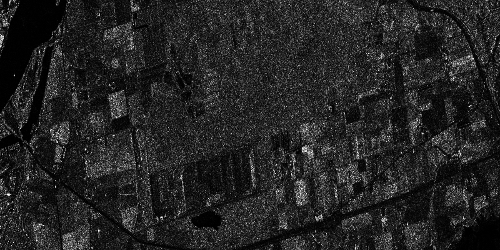
\includegraphics[width=\textwidth]{../Art/test-left-co-2.png}
    \itkcaption[SAR polarimetry conversion]{Image LL (sensor : RADARSAT2).}
    \label{fig:polsynthll}
   \end{figure}
   
   \begin{figure}[h!]
    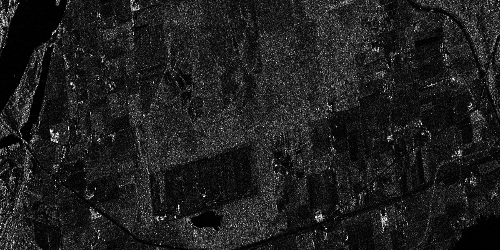
\includegraphics[width=\textwidth]{../Art/test-left-cross-2.png}
    \itkcaption[SAR polarimetry conversion]{Image LR (sensor : RADARSAT2).}
    \label{fig:polsynthlr}
   \end{figure}
\end{center}


\subsubsection{Polarimetric data visualization}

Finally, let's talk about polarimetric data visualization. There is a strong link between polarimetric data visualization and the way they can be decomposed into significant physical processes.
Indeed, by setting the results (or combinations) of such decompositions to RGB channels, it is possible to obtain nice colorations that help in interpreting SAR polarimetric images.

There is no specific dedicated application yet, but it is possible to use a combination of different applications as a replacement.
Let's do it with a RADARSAT2 acquisition over the famous place of the Golden Gate Bridge, San Francisco, California.

We first extract a ROI from the original image (not required). 


\begin{itemize}
\item 
\begin{verbatim} 
otbcli_ExtractROI -in imagery_HH.tif -out
  imagery_HH_extract.tif -startx 0 -starty 6300 -sizex 2790 -sizey 2400 
\end{verbatim}
									  
\item 
\begin{verbatim} 
otbcli_ExtractROI -in imagery_HV.tif -out
  imagery_HV_extract.tif -startx 0 -starty 6300 -sizex 2790 -sizey 2400 
\end{verbatim}
									  
\item 
\begin{verbatim} 
otbcli_ExtractROI -in imagery_VV.tif -out
  imagery_VV_extract.tif -startx 0 -starty 6300 -sizex 2790 -sizey 2400 
\end{verbatim}
\end{itemize}

Then we need to obtain the amplitude of each band; BandMath is the application we want :

\begin{itemize}
\item 
\begin{verbatim} 
otbcli_BandMath -il imagery_HH_extract.tif -out HH.tif -exp
"sqrt(im1b1^2+im1b2^2)" 
\end{verbatim}
									  
\item 
\begin{verbatim} 
otbcli_BandMath -il imagery_HV_extract.tif -out HV.tif
  -exp "sqrt(im1b1^2+im1b2^2)" 
\end{verbatim}
									  
\item 
\begin{verbatim} 
otbcli_BandMath -il imagery_VV_extract.tif -out VV.tif
  -exp "sqrt(im1b1^2+im1b2^2)" 
\end{verbatim}
\end{itemize}

Note that BandMath application interprets the image 'imagery\_XX\_extract.tif' as an image made of two bands, where the first one is related to the real part of the signal,
and where the second one is related to the imaginary part (that's why the modulus is obtained by the expressions $im1b1^2+im1b2^2$).


We then rescale the produced images to intensities ranging from 0 to 255 :

\begin{itemize}
\item 
\begin{verbatim} 
otbcli_Rescale -in HH.tif -out HH_res.png uint8 
\end{verbatim}
									  
\item 
\begin{verbatim} 
otbcli_Rescale -in HV.tif -out HV_res.png uint8 
\end{verbatim}
									  
\item 
\begin{verbatim} 
otbcli_Rescale -in VV.tif -out VV_res.png uint8 
\end{verbatim}
\end{itemize}

The three figures below (\ref{fig:hhfrisco} , \ref{fig:hvfrisco} and \ref{fig:vvfrisco}) show the images obtained :

\begin{center}
  \begin{figure}[h!]
    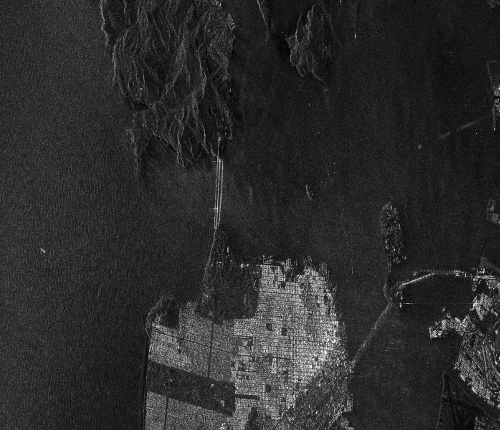
\includegraphics[width=\textwidth]{../Art/RSAT2_HH_Frisco.png}
    \itkcaption[SAR polarimetry visu]{Band HH in amplitude (sensor : RADARSAT2).}
    \label{fig:hhfrisco}
   \end{figure}
   
   \begin{figure}[h!]
    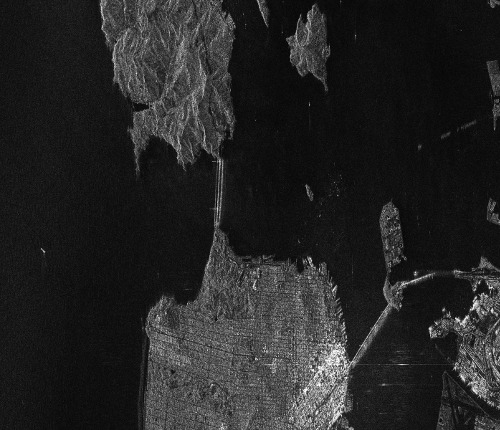
\includegraphics[width=\textwidth]{../Art/RSAT2_HV_Frisco.png}
    \itkcaption[SAR polarimetry visu]{Band HV in amplitude (sensor : RADARSAT2).}
    \label{fig:hvfrisco}
   \end{figure}
      
   \begin{figure}[h!]
    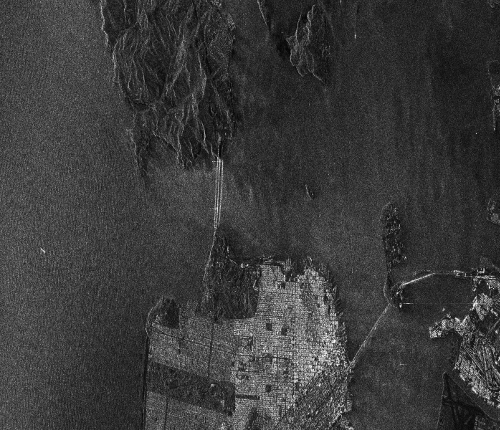
\includegraphics[width=\textwidth]{../Art/RSAT2_VV_Frisco.png}
    \itkcaption[SAR polarimetry visu]{Band VV in amplitude (sensor : RADARSAT2).}
    \label{fig:vvfrisco}
   \end{figure}
\end{center}


Now the most interesting step. In order to get a friendly coloration of these data, we are going to use the Pauli decomposition,
defined as follows :

\begin{itemize}
\item  $a=\frac{|S_{HH}-S_{VV}|}{\sqrt{2}}$ 
									  
\item  $b=\sqrt{2}.|S_{HV}|$ 
									  
\item  $c=\frac{|S_{HH}+S_{VV}|}{\sqrt{2}}$ 
\end{itemize}

We use the BandMath application one again :

\begin{itemize}
\item 
\begin{verbatim} 
otbcli_BandMath -il imagery_HH_extract.tif
  imagery_HV_extract.tif imagery_VV_extract.tif -out Channel1.tif -exp
  "sqrt(((im1b1-im3b1)^2+(im1b2-im3b2)^2))" 
\end{verbatim}
									  
\item 
\begin{verbatim} 
otbcli_BandMath -il imagery_HH_extract.tif
  imagery_HV_extract.tif imagery_VV_extract.tif -out Channel2.tif -exp
  "sqrt(im2b1^2+im2b2^2)" 
\end{verbatim}
									  
\item 
\begin{verbatim} 
otbcli_BandMath -il imagery_HH_extract.tif imagery_HV_extract.tif
imagery_VV_extract.tif -out Channel3.tif -exp
"sqrt(((im1b1+im3b1)^2+(im1b2+im3b2)^2))" 
\end{verbatim}
\end{itemize}

Note that sqrt(2) factors have been omitted purposely, since their effects will be canceled by the rescaling step.


We then rescale the produced images to intensities ranging from 0 to 255 :

\begin{itemize}
\item 
\begin{verbatim} 
otbcli_Rescale -in Channel1.tif -out Channel1_res.tif uint8 
\end{verbatim}
									  
\item 
\begin{verbatim} 
otbcli_Rescale -in Channel2.tif -out Channel2_res.tif uint8 
\end{verbatim}
									  
\item 
\begin{verbatim} 
otbcli_Rescale -in Channel3.tif -out Channel3_res.tif uint8 
\end{verbatim}
\end{itemize}

And finally, we merge the three bands into a single RGB image.

\begin{verbatim} 
otbcli_ConcatenateImages -il Channel1_res.tif Channel2_res.tif Channel3_res.tif
-out visuPauli.png 
\end{verbatim}

The result is shown in the figure below (\ref{fig:colorfrisco}).

\begin{center}
  \begin{figure}[h!]
    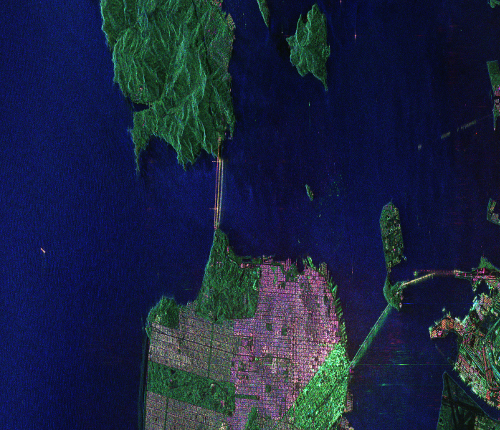
\includegraphics[width=\textwidth]{../Art/visuPauli.png}
    \itkcaption[SAR polarimetry visu]{RGB image obtained from Pauli decomposition (sensor : RADARSAT2).}
    \label{fig:colorfrisco}
   \end{figure}
\end{center}
